\section{Home Assistant}
\label{sec:homeassistant}
    Eines der populärsten \acl{SH} Plattformen ist das sogenannte Home Assistant System. Die Open-Source-Software ist ein zentrales 
    Steuerungssystem von Heimautomationen und der Verwaltung von intelligenten Geräten mit dem Fokus der lokalen Steuerung und gesicherter 
    Privatsphäre. Der Zugriff kann über die Smartphone-App, jeweils verfügbar für iOS und Android, oder auch über die webbasierte 
    Benutzeroberfläche (Web-App) erfolgen. In dem lokalen System können auch Geräte die Steuerung per Sprachbefehlen ermöglichen. Kompatible 
    Plattformen sind unter anderem Google Assistant, Amazon Alexa und Apple HomeKit. Dies sind weitaus nur eine Selektion von bekannten 
    Herstellern. Home Assistant bietet eine weitaus vielfältigere Verknüpfung von Geräten, Services und Plattformen. Die zentrale Steuerung 
    unterstützt durch modulare Integrationskomponenten die einzelnen Geräte, Anwendungen und Services. Für die drahtlose Kommunikation 
    werden native Integrationskomponenten verwendet, darunter Bluetooth, ZigBee und Z-Wave. Diese werden verwendet, um lokale \ac{PAN} mit 
    Geräten mit geringem Stromverbrauch aufzubauen. Die Steuerung kann auch mit Proprietären Ökosystemen stattfinden, sofern diese eine offene 
    \acs{API} oder Anbindungen über \acs{MQTT} anbieten.\footnote{Grundlegende Ableitung der Definition von Home Assistant siehe \url{https://en.wikipedia.org/wiki/Home_Assistant} Abgerufen am 16.04.2022}
    \\
    Die Platform ist in Python geschrieben und wird aktiv instand gehalten und durch eine große Community unterstützt. Die Software ist allgemein unter 
    der Apache 2.0, veröffentlicht. Der folgende Abschnitt befasst sich in Kürze mit der Historie des Systems. 
    
    \subsection*{Historie}
    \label{sec:historyHOAS}
        Anfang des vierten Quartals im Jahr 2013 startete das Python-Projekt von Paulus Schoutsen und im November 2013 erstmals auf GitHub 
        veröffentlicht.\footnote{Anfänge von Home Assistant. \url{https://www.linux.com/topic/embedded-iot/home-assistant-python-approach-home-automation/} Abgerufen am 18.04.2022}
        \\
        \linebreak
        Vier Jahre nach den ersten Entwicklungen der \acl{SH} Plattform wurde im Juli 2017 ein verwaltetes Betriebssystem mit dem Namen 
        \textit{Hass.io} entwickelt.\footnote{Verkündungen von Home Assistant. \url{https://www.home-assistant.io/blog/categories/announcements/} Abgerufen am 18.04.2022} 
        Dadurch gelang der Durchbruch der vereinfachten Verwendung von der Home Assistant Plattform auf kleineren Computern, sogenannten 
        Einplatinencomputern, wie beispielsweise einem der Raspberry Pi Serie. In Zusammenhang mit dem Betriebssystem kam ein 
        \textit{Supervisor}-Verwaltungssystem hinzu, das den Benutzern die Verwaltung, Sicherung und Aktualisierung der lokalen Installation 
        ermöglicht. Ein weiteres Feature des Supervisors ist die Möglichkeit der Plattform über Add Ons weitere Funktionalitäten zu Verfügung zu 
        stellen.\footnote{Einstieg in das Hass.io Betriebssystem. \url{https://www.home-assistant.io/blog/2017/07/25/introducing-hassio/} Abgerufen am 18.04.2022}
        \\
        \linebreak
        Die Software wird stetig weiterentwickelt und verbessert. Mittlerweile gehört sie zu den am meist genutzten Open-Source-Plattformen 
        im Bereich \acl{SH}.

\subsection{Konzept und Architektur}
\label{sec:conceptArchitectureHAOS}
    Home Assistant bietet eine Plattform für die zentrale Haussteuerung und die damit einhergehende Steuerung von Heimautomationen. Die 
    Software ist nicht nur eine einfache Steuerungs- und Konfigurations-Software, sondern ein eingebettetes Betriebssystem, das 
    verbraucher- und nutzerorientiert das Verwenden und Konfigurieren von Haussteuerungen erleichtert. \footnote{Konzept und Architektur von Home Assistant. \url{https://developers.home-assistant.io/docs/architecture_index} Abgerufen am 19.04.2022}
    \\
    \linebreak
    Damit der offene Ansatz von Home Assistant Anbietern gegenüber nicht eingeschränkt ist, bietet die Software Möglichkeiten, um viele 
    Geräte zu vereinheitlichen. Somit begegnet Home Assistant der Heterogenität des offenen Marktes, in sofern, dass diese Geräte auf ein 
    gemeinsame Konzepte gebracht werden. Diese sind in vier Konzepte\footnote{Erläuterung der Konzepte von Home Assistant. \url{https://apiumhub.com/tech-blog-barcelona/domotics-with-home-assistant-concepts/} Abgerufen am 21.04.2022} 
    aufgeteilt, mit der die Vereinheitlichung vorangetrieben werden kann: 
    \begin{itemize}
        \item Integration (Integration): Integrationen repräsentieren die Geräte und Dienste innerhalb der Home Assistant Anwendung. 
              Ebenso können mittels den Integrationen auch Daten von Datenpunkten abgerufen werden.
        \item Gerät (Device): Nach der Konfiguration der Integration werden die Geräte in Home Assistant angelegt. 
              Diese werden dann als erkannte Geräte der Integration dargestellt, z.B. als Temperatur-, Licht- oder Feuchtigkeitssensor.
        \item Entität (Entity): Die Datenpunkte sind die Geräte, die sogenannten Entitäten, die durch die Integrationen standardisiert werden. 
              Dies sin Objekte, die Funktionalitäten oder Daten des Geräts darstellen, z.B. die Temperatur, Helligkeit oder die Feuchtigkeit.
        \item Automatisierung (Automation): Automatisierungen sind Prozesse, die bei einem bestimmten ausgelösten Event ausgeführt werden 
              sollen. Dieses Auslöser (trigger) können Zeitpunkte, Ereignisse oder manuell gesteuerte Aktionen des Nutzers sein, z.B. das 
              Ausschalten des Bürolichts, wenn durch einen Bewegungssensor fünf Minuten keine Bewegung festgestellt wurde oder wenn der 
              Helligkeitswert, der über den Sensor festgestellt wurde einen bestimmten Wert erreicht hat, soll das Licht ebenso 
              ausgeschaltet werden.
    \end{itemize}
    Die Architektur der Home Assistant Anwendung ist grundlegend als eingebettetes System eines Betriebssystem aufgestellt, welches in 
    drei Schichten aufgeteilt ist. In unterster Ebene befindet sich das Betriebssystem, welches als minimales Linux System aufgestellt 
    ist, um die darauf liegenden Schichten, den Aufseher (supervisor) und den Kern (core), zu betreiben. Mit dem Supervisor wird das 
    Betriebssystem verwaltet und konfiguriert. Der eigentliche Kern interagiert mit dem Supervisor, den Geräten und den Services. 
    %Erläuterung supvervisor und core Architektur
    \\
    \linebreak
    Der Supervisor ist die Schicht über dem Betriebssystem, die über einen D-Bus kommunizieren. Diese Zwischenschicht ermöglicht dem 
    Benutzer die Verwaltung der Home Assistant Installation. Die Aufgaben des Supervisors sind wie folgt 
    definiert\footnote{Architektur der Home Assistant Software. \url{https://developers.home-assistant.io/docs/supervisor} Abgerufen am 22.04.2022}: 
    \begin{itemize}
        \item Dieser führt den Home Assistant Kern (Core) aus.
        \item Dieser führt die Updates des Home Assistant Core aus.
        \item Dieser führt einen \textit{Rollback} bei Fehlgeschlagenem Update durch.
        \item Dieser führt Sicherungen und Wiederherstellungen durch.
        \item Dieser verwaltet die Add Ons der Core Instanz
    \end{itemize}
    \begin{figure}
        \centering
        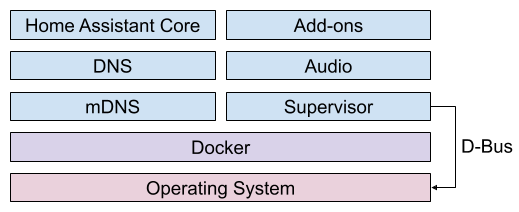
\includegraphics[width=10cm,height=10cm,keepaspectratio]{images/ha_architecture_2020.png}
        \caption{Architektur des Home Assistant Supervisors}
        \label{fig:architectureHAOS}
    \end{figure}

    Die auf dem Supervisor aufbauende Architektur ist die Architektur der Anwendung, der sogenannte Core. 

    %Die Übersicht über die HA-Architektur ist in Abb. 1 dargestellt. HA besteht aus vier Hauptteilen: Event Bus, State Machine, Service 
    %Registry und Timer. Der Event Bus ist die zentrale Komponente des HA, der verwendet wird, um das Auslösen und Abhören von Ereignissen 
    %zu erleichtern. Die Zustandsmaschine kann den Zustand von Dingen überwachen und löst ein Zustandsänderungsereignis an Event Bus aus, 
    %sobald ein Zustand aktualisiert wurde. Die Dienstregistrierung ist dafür verantwortlich, den Ereignisbus auf Anrufdienstereignisse 
    %abzuhören. Benutzer können einen Dienst über die Dienstregistrierung hinzufügen. Automatisierung und Dienst „Entwicklertools“ im 
    %Frontend können Dienste aufrufen. Der Timer ist angepasst, um ein zeitverändertes Ereignis gemäß einer gegebenen Frequenz auf dem 
    %Ereignisbus zu senden. Diese Komponente vereinfacht die Automatisierung basierend auf der Dauer. HA verwendet SQLite als Datenbank, 
    %was bedeutet, dass keine Cloud Daten über das Leben des Benutzers sammelt. Nur der Benutzer kann auf den Zustand des Hauses zugreifen. 
    %Außerdem wird die Kommunikation mit dem Gateway verschlüsselt. Der HA bietet jedoch eine Verlaufskomponente, die alles verfolgen kann, 
    %was sich innerhalb der Plattform ereignet. Somit können Nutzer auf alle gespeicherten Informationen zu Hause zugreifen.
    
    % Beschreibung der Konzepte und Architektur von Home Assistant.
    %Bild der Architektur
    % Beschreibung der Komponenten, Aufbau etc von Home Assistant
%\subsection{Architektur}

\subsection{Ziele und Schwerpunkte}
    %https://apiumhub.com/tech-blog-barcelona/domotics-with-home-assistant-concepts/
    %Home Assistant is created to address these issues:
    %– Could we have a single home automation/control centre, compatible with almost all electronic devices?
    %– Could we make the sending of data to an external server visible? Could we even eliminate it completely?

\subsection{Stärken und Schwächen}
